\documentclass[11pt]{article}

\usepackage[a4paper,margin=24mm]{geometry}
\usepackage{amsmath}
\usepackage{graphicx}
\usepackage{booktabs}
\usepackage{array}
\usepackage{xcolor}
\usepackage{enumitem}
\usepackage{titlesec}
\usepackage{fancyhdr}
\usepackage[hidelinks]{hyperref}
\usepackage{longtable}

\definecolor{ink}{HTML}{222222}
\definecolor{accent}{HTML}{0072B2}
\definecolor{old}{HTML}{B0632A}
\definecolor{ok}{HTML}{009E73}
\definecolor{rule}{HTML}{DDDDDD}

\color{ink}
\titleformat{\section}{\Large\bfseries\color{accent}}{\thesection}{0.6em}{}
\titleformat{\subsection}{\large\bfseries}{\thesubsection}{0.6em}{}
\setlist{itemsep=2pt,topsep=3pt,parsep=0pt}
\renewcommand{\arraystretch}{1.25}

\pagestyle{fancy}\fancyhf{}
\lhead{\small\color{accent}OptiComp2}
\rhead{\small Changes vs.\ the original OptiComp}
\cfoot{\small\thepage}
\renewcommand{\headrulewidth}{0.4pt}

\newcommand{\yes}{\textcolor{ok}{\textbf{yes}}}
\newcommand{\no}{\textcolor{old}{no}}
\newcommand{\code}[1]{\texttt{\small #1}}

\begin{document}

\thispagestyle{empty}
\vspace*{2.2cm}
\begin{center}
{\Huge\bfseries\color{accent} OptiComp2}\\[6pt]
{\LARGE\bfseries Change list relative to the original OptiComp}\\[16pt]
{\large A clean-room rewrite of the angle-resolved spectrophotometer control software}\\[10pt]
{\large with performance and reliability improvements}\\[26pt]
{\large Haoxiang Zhang}\\[6pt]
{\normalsize August 2026}\\[4pt]
{\normalsize Original: OptiComp v1.3.3 \quad$\rightarrow$\quad OptiComp2}
\end{center}
\vfill
\noindent\small
This document lists the changes OptiComp2 makes relative to the original \emph{OptiComp} control
software, and quantifies the resulting improvements in code coverage, measurement reliability and
data quality. The original repository was \textbf{not modified in any way}; OptiComp2 is an
independent rewrite that lives in its own folder and repository and runs on the same instrument.
\newpage

\tableofcontents
\newpage

\section{Overview and approach}

The original OptiComp (v1.3.3, Python~3.9 + Tkinter, 11 modules, about 1\,800 lines) drove the
angle-resolved spectrophotometer (the VAR/ARS system): a Thorlabs Elliptec rotation-stage assembly
(shutter, polariser, detector arm and sample stage on a shared serial bus) and a B\&W~Tek
spectrometer accessed through \code{BWTEKUSB.dll}.

A function-level review of the original software on 2026-08-25 produced 35~findings, all
adversarially verified. Rather than patch the original in place, the software was rewritten
clean-room in the order \emph{protocol layer $\rightarrow$ spectrometer $\rightarrow$ measurement
sequence $\rightarrow$ analysis $\rightarrow$ GUI}, validating each layer at the instrument. The
result, OptiComp2, keeps the original's calibrated geometry and measurement model but adds command
verification, saturation handling, automatic integration-time calibration, hardware-recovery paths,
persistent motor-state bookkeeping and a full unit-test suite.

\section{At a glance}

\begin{figure}[h]
\centering
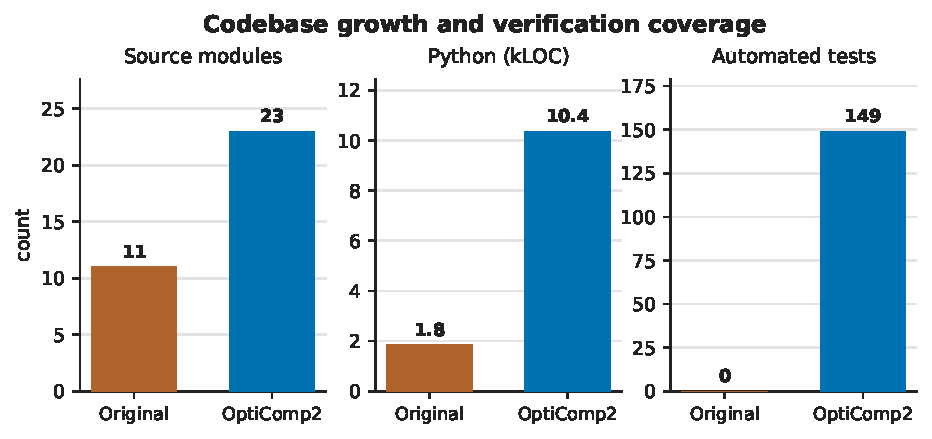
\includegraphics[width=\linewidth]{figures/fig_codebase.pdf}
\end{figure}

\noindent The rewrite is roughly $5.6\times$ the original in Python source and, for the first time,
ships an automated test suite (149~tests, all runnable without hardware against fake serial and DLL
back-ends). The added surface is almost entirely verification, recovery and safety logic rather than
new measurement features.

\begin{figure}[h]
\centering
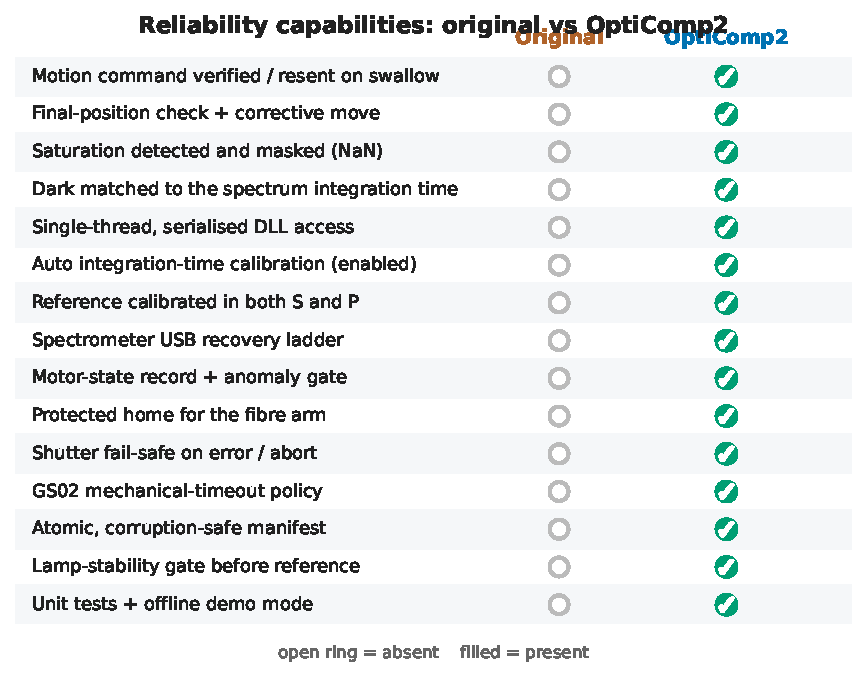
\includegraphics[width=\linewidth]{figures/fig_capability.pdf}
\end{figure}

\noindent Every capability above is absent in the original and present in OptiComp2. Sections~4 and~5
describe each one and the failure it prevents.

\begin{figure}[h]
\centering
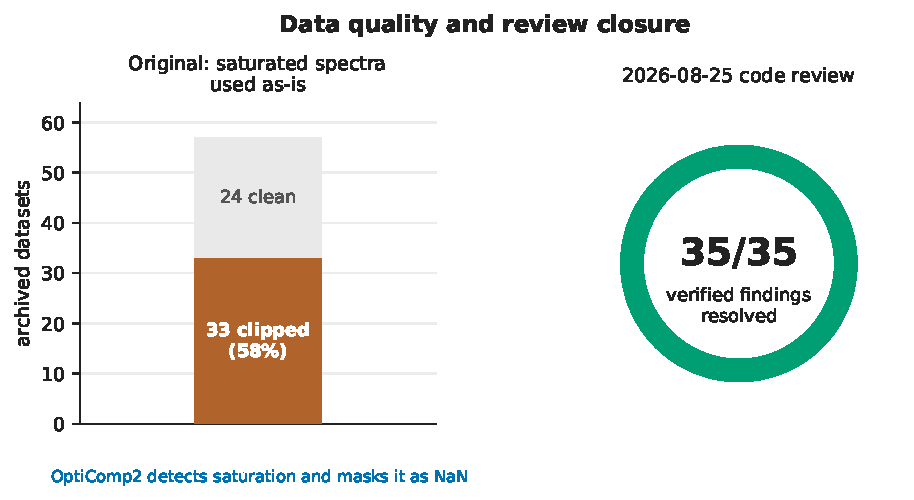
\includegraphics[width=0.92\linewidth]{figures/fig_dataquality.pdf}
\end{figure}

\noindent In the original data, 33 of 57 archived datasets (58\,\%) contain spectra clipped at the
16-bit full scale that the original pipeline used without flagging, because the integration time was
fixed (\code{HARD\_IT}) with no saturation check. OptiComp2 detects saturation and records the
affected pixels as \code{NaN} so they cannot enter a reflectance. All 35 review findings are
resolved.

\section{What the review of the original found}

The changes in the following sections address these verified defects of the original software.

\begin{enumerate}[label=\textbf{R\arabic*.}]
\item \textbf{Motion commands were not verified.} About 4\,\% of \code{ma} commands to the ELL18
sample stage are silently swallowed (no reply, no motion, then \code{GS00}). The original never
checked the final position, so angle-wrong spectra may exist in the old data.
\item \textbf{Saturation was not detected.} A fixed \code{HARD\_IT} with no saturation check left
33 of 57 archived datasets with clipped spectra (Figure in \S2).
\item \textbf{Dark integration-time mismatch.} \code{Dark.csv} was taken at a fixed 1000\,ms while
the VAR spectra used \code{HARD\_IT}, so the dark subtraction was not rigorous.
\item \textbf{Concurrent DLL calls.} The GUI thread and the scan thread called \code{BWTEKUSB.dll}
concurrently with no declared thread safety.
\item \textbf{Off-by-one active-pixel slice.} The thesis specifies pixels 254--2030 inclusive; the
code sliced 1776 pixels, dropping pixel 2030.
\item \textbf{Scan gatekeeper incomplete.} The original checked the 0--80$^\circ$ start/stop bounds
but never validated step $\ge 1$ (a zero or negative step passed the gate). OptiComp2 enforces
$0 \le \text{start} < \text{stop} \le 80$ with step $\ge 1$.
\item \textbf{Reference integration-time calibration disabled.} The reference calibration at
80$^\circ$ (thesis \S4.2.3.3) survived only as commented-out code and a never-called setter; a fixed
\code{HARD\_IT} was used in practice.
\item \textbf{Inconsistent sample-stage offset.} One module used 103$^\circ$, another 105$^\circ$
(the VAR scan actually used 105$^\circ$).
\end{enumerate}

The review also confirmed that the polarisation file labels in the archived data are in fact
\emph{correct} (the \code{\_P\_} datasets show the expected Brewster minimum); only a single
polarisation-mode label in the original UI was reversed relative to the files. OptiComp2 keeps the
verified file convention.

\section{Layer-by-layer changes}

\subsection{Elliptec protocol layer (\code{hw/elliptec.py})}
\begin{longtable}{>{\raggedright\arraybackslash}p{0.46\linewidth} >{\raggedright\arraybackslash}p{0.48\linewidth}}
\toprule
\textbf{Original behaviour (measured)} & \textbf{OptiComp2} \\
\midrule\endhead
A command is occasionally swallowed (no reply, no motion). &
Read the position first; on no reply, poll \code{GS}; if the position has not changed,
\textbf{resend}, up to three times. \\
After a long move the stage stops a few hundredths of a degree short. &
Within $\pm20$ pulses (0.05$^\circ$) counts as on-target; up to 120 pulses (0.3$^\circ$) issues a
\textbf{corrective move}; beyond that, accept with a warning or raise an error. \\
\code{PO} returns only at end of motion; an ELL18 move at 50\,\% takes $>5$\,s. &
Poll \code{GS} after an initial 2\,s wait; 60\,s motion timeout. \\
Reply lines truncated by the read timeout were decoded. &
Any line without a terminator or with a wrong-length payload is discarded, never decoded. \\
A mechanical timeout (\code{GS02}) was retried blindly. &
\code{ma}/\code{fw}/\code{bw} retry with backoff; \code{mr} is reissued as an absolute \code{ma} to
the original target; \textbf{\code{ho} never retries}. \\
Homing the fibre arm (module~2) could tangle the fibre. &
\code{protected\_home}: \code{home("2")} requires \code{force=True}, and the raw channel refuses to
send \code{ho} to a protected address. \\
Module type and pulse count were hard-coded. &
Model, serial, travel and pulses/rev are read from the \code{IN} reply. \\
\bottomrule
\end{longtable}

\subsection{Spectrometer (\code{hw/bwtek.py})}
\begin{itemize}
\item Every DLL call sets \code{argtypes}/\code{restype} and checks the return code; \code{read()}
logs a warning on an anomalous duration.
\item \textbf{Automatic integration time}: target the peak at 85\,\% of full scale, accept band
78--92\,\%, linear extrapolation, halve on saturation, at most eight steps. If there is still no
light at the hardware ceiling it \textbf{aborts with a diagnostic} instead of carrying over a
non-converged integration time (Figure~\ref{fig:autoit}).
\item \textbf{Reference calibrated in both S and P, keeping} $\min(\mathrm{IT}_S,\mathrm{IT}_P)$: on a
diffuse white reference the P channel is about 12\,\% brighter than S, so calibrating in a single
polarisation (as the original procedure did) would saturate the brighter P spectra.
\item \textbf{Recovery ladder} \code{recover()}: close $+$ reopen, then a PnP restart of only the
spectrometer USB device (equivalent to a replug, but it does not touch the hub the bus board shares).
\item Saturated pixels are masked as \code{NaN} in the analysis; darks are stored per integration
time and matched to the spectrum.
\end{itemize}

\begin{figure}[h]
\centering
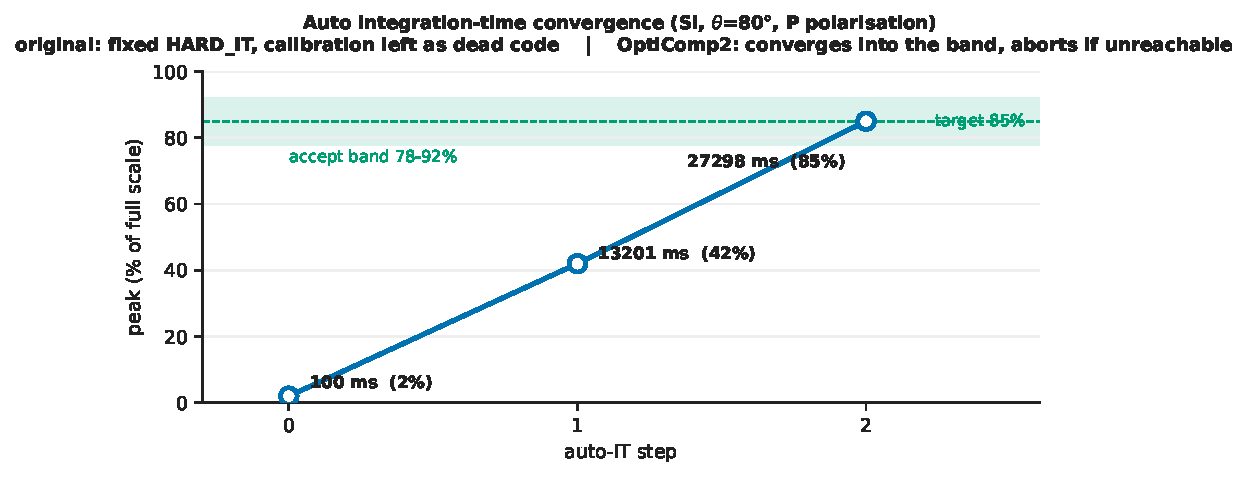
\includegraphics[width=0.96\linewidth]{figures/fig_autoit.pdf}
\caption{Automatic integration-time calibration converging on a dim target from a cold start. The
original left this calibration as dead code and used a fixed \code{HARD\_IT}; OptiComp2 drives the
peak into the 78--92\,\% accept band, announces multi-second exposures so a long read is not mistaken
for a hang, and aborts cleanly if the band is unreachable even at the hardware ceiling.}
\label{fig:autoit}
\end{figure}

\subsection{Motor-state record (\code{hw/stagestate.py}, new)}
\begin{itemize}
\item After every move the sequence records that module's position and status; on disconnect/exit a
full snapshot of all four modules is written to \code{data/stage\_state.json}.
\item On every connect and script start the state is compared against the baseline: a position
difference $>0.5^\circ$, a non-zero status code, or a changed speed is flagged. Unattended scripts
abort on an anomaly (and refuse even with \code{--force} when the detector arm reports \code{GS02});
the GUI shows a banner but does not block manual operation.
\item The detector-arm speed is reset to 50\,\% on connect (a module reverts to its 64\,\% default
after a power loss).
\end{itemize}

\subsection{Measurement sequence (\code{tools/sequence.py})}
\begin{itemize}
\item Step primitives (\code{stage}, \code{shutter}, \code{set\_it}, \code{auto\_it}, \code{acquire},
\code{pause}, \dots) and builders: reference calibration, dark, single angle, angle scan and
double-beam.
\item The Runner enforces soft limits (0--200$^\circ$), detects motion ``not by us'' before a move,
closes the shutter on any error or abort, and writes \code{manifest.json} atomically (temp file $+$
\code{os.replace}); an unreadable manifest is moved aside rather than overwritten.
\item Gatekeeper: $0 \le \text{start} < \text{stop} \le 80$, step $\ge 1$; when unattended, a
\code{pause} aborts rather than waiting forever.
\end{itemize}

\subsection{Analysis (\code{analysis/})}
\begin{itemize}
\item Reflectance by the double-beam substitution relation, with darks matched by integration time
(and normalised by counts/ms with a recorded note if they differ).
\item Active pixels 254--2030 inclusive (1777 pixels), fixing the off-by-one.
\item Standards: constant (white reference), a silicon Fresnel table (real $n$, marked invalid below
380\,nm), BK7 Sellmeier, and a slab back-surface inversion. Invalid wavelengths and masked pixels are
exported as \code{NaN}, never as a physically meaningless reflectance.
\end{itemize}

\subsection{GUI (\code{tools/manual\_gui.py})}
\begin{itemize}
\item A five-page sidebar layout (instrument, motors \& shutter, spectrometer, measurement,
analysis), a persistent status bar and a red ``close shutter'' reachable from any page.
\item Manual controls are locked while a sequence runs; the exit flow aborts the run, closes the
shutter and records state within a bounded time.
\item An offline \textbf{demo mode} (\code{--demo}) drives the whole GUI against fake hardware without
touching the serial port or the DLL, which is also what the test suite and the layout audit use.
\end{itemize}

\subsection{Operational tools (new)}
\begin{center}
\begin{tabular}{>{\raggedright\arraybackslash}p{0.24\linewidth} >{\raggedright\arraybackslash}p{0.68\linewidth}}
\toprule
\textbf{Tool} & \textbf{Purpose} \\
\midrule
\code{restore\_stages.py} & Read-only bus report; \code{-{}-safe -{}-arm} restores the stage
reference under supervision and writes the baseline. \\
\code{usb\_reset.py} & Probe or PnP-restart the spectrometer USB device. \\
\code{shutter\_close.py} & After a hard-killed script: close the shutter and verify position 0. \\
\code{monitor.py} & Unattended stability monitor (continuous reads at a fixed geometry). \\
\code{cycle\_test.py} & Motion-cycle test with automatic recovery. \\
\code{ell\_probe.py}, \code{spec\_probe.py} & Read-only probes. \\
\bottomrule
\end{tabular}
\end{center}

\section{Reliability hardening added after the rewrite}

Beyond the layer-by-layer parity work, several rounds of hardening were applied and each is covered by
a regression test:

\begin{itemize}
\item \textbf{Eleven pipeline fixes} against unattended-run failures, including: the shutter is marked
open \emph{before} the open command so a mid-open failure is still closed by the safety path; the GUI
event pumps re-arm in a \code{finally} so one handler exception cannot freeze the interface; the USB
device-ID parser is locale-independent so recovery works on a non-English Windows; and a corrupt
manifest that parses as a non-dictionary no longer raises.
\item \textbf{Lamp-stability gate} (optional, on by default) before the reference calibration: the
active-band mean must hold within 0.5\,\% for five consecutive reads, so lamp drift between the
reference and sample sessions cannot bias the reflectance. It warns and proceeds rather than blocking.
\item \textbf{Auto-integration-time ceiling}: a target too dim to reach the accept band even at the
60\,s hardware limit now fails after a single ceiling read with a diagnostic (reference / lamp /
fibre / shutter), instead of repeating multi-second reads that resemble a hang. Legitimately dim
references (for example silicon at 80$^\circ$ in P, which calibrates at tens of seconds) still
converge, and any long exposure is announced.
\end{itemize}

\section{Deliberately not carried over}

Some behaviours of the original were intentionally left out because they were unused, broken, or out
of scope for a single-operator instrument. These are listed for completeness; none affects the VAR
measurement:

\begin{itemize}
\item Fixed-window (boxcar) smoothing applied before storage --- OptiComp2 stores raw counts and
smooths only for display.
\item Dead or partial acquisition modes not part of the VAR workflow.
\item A wavelength-correction path that did not match the calibration.
\item The administrator gate and multi-user working directories.
\end{itemize}

\noindent (The exact original inventory is in the repository review notes; the point is that the VAR
acquisition, geometry and analysis are fully reproduced and improved.)

\section{Verification and deployment}

\begin{itemize}
\item \textbf{Tests}: 149 unit tests, passing both on a workstation and on the instrument PC
(\code{py -m unittest discover -s tests}, no third-party test runner needed). They cover protocol
encode/decode, truncated replies, resend and corrective moves, protected home, DLL return codes and
the PnP-restart safety, Runner safety (an abort closes the shutter, soft limits, the unattended-pause
abort), monitor/cycle fault-injection recovery, state comparison, and a GUI feature-reference and
layout audit driven against the demo hardware.
\item \textbf{Deployment}: code directories are copied to the instrument PC and a full test run is
done there after each deployment; the raw measurement data and standards on the instrument are never
overwritten.
\item \textbf{Live validation}: the four Elliptec modules enumerate with the detector arm unmoved, the
spectrometer reads a healthy frame, and the full demo workflow runs end-to-end including the dim
silicon calibration case.
\end{itemize}

\vspace{1em}
\noindent\rule{\linewidth}{0.4pt}\\[4pt]
\small\emph{Summary.} OptiComp2 reproduces the original VAR measurement and geometry while adding
command verification, saturation handling, automatic integration-time calibration in both
polarisations, hardware-recovery paths, persistent motor-state safety and a 149-test suite ---
turning a fixed-exposure, unverified acquisition into a self-checking one whose failures are explicit
and recoverable.

\end{document}
